
% Copyright (c) 2015 - 2020 Mario Mlačak, mmlacak@gmail.com
% Licensed and published as Public Domain work.

% Mayan Ascendancy chapter ============================================
\chapter*{Mayan Ascendancy}
\addcontentsline{toc}{chapter}{Mayan Ascendancy}

\begin{flushright}
\parbox{0.8\textwidth}{
\emph{The world has achieved brilliance without wisdom, power without
conscience. Our is a world of nuclear giants and ethical infants. \\
\hspace*{\fill}{\textperiodcentered \textperiodcentered \textperiodcentered \hspace*{0.2em} Omar Nelson Bradley} } }
\end{flushright}

\noindent
Mayan Ascendancy is chess variant which is played on 12 x 12 board with
yellow and blue fields and with dark yellow and dark blue pieces. In
algebraic notation, columns are enumerated from 'a' to 'l', and rows are
enumerated from '1' to '12'. A new piece is introduced, Pyramid.

\clearpage % ..........................................................
% Pyramid *************************************************************

\section*{Pyramid}
\addcontentsline{toc}{section}{Pyramid}

\noindent
\begin{wrapfigure}[12]{l}{0.4\textwidth}
\centering
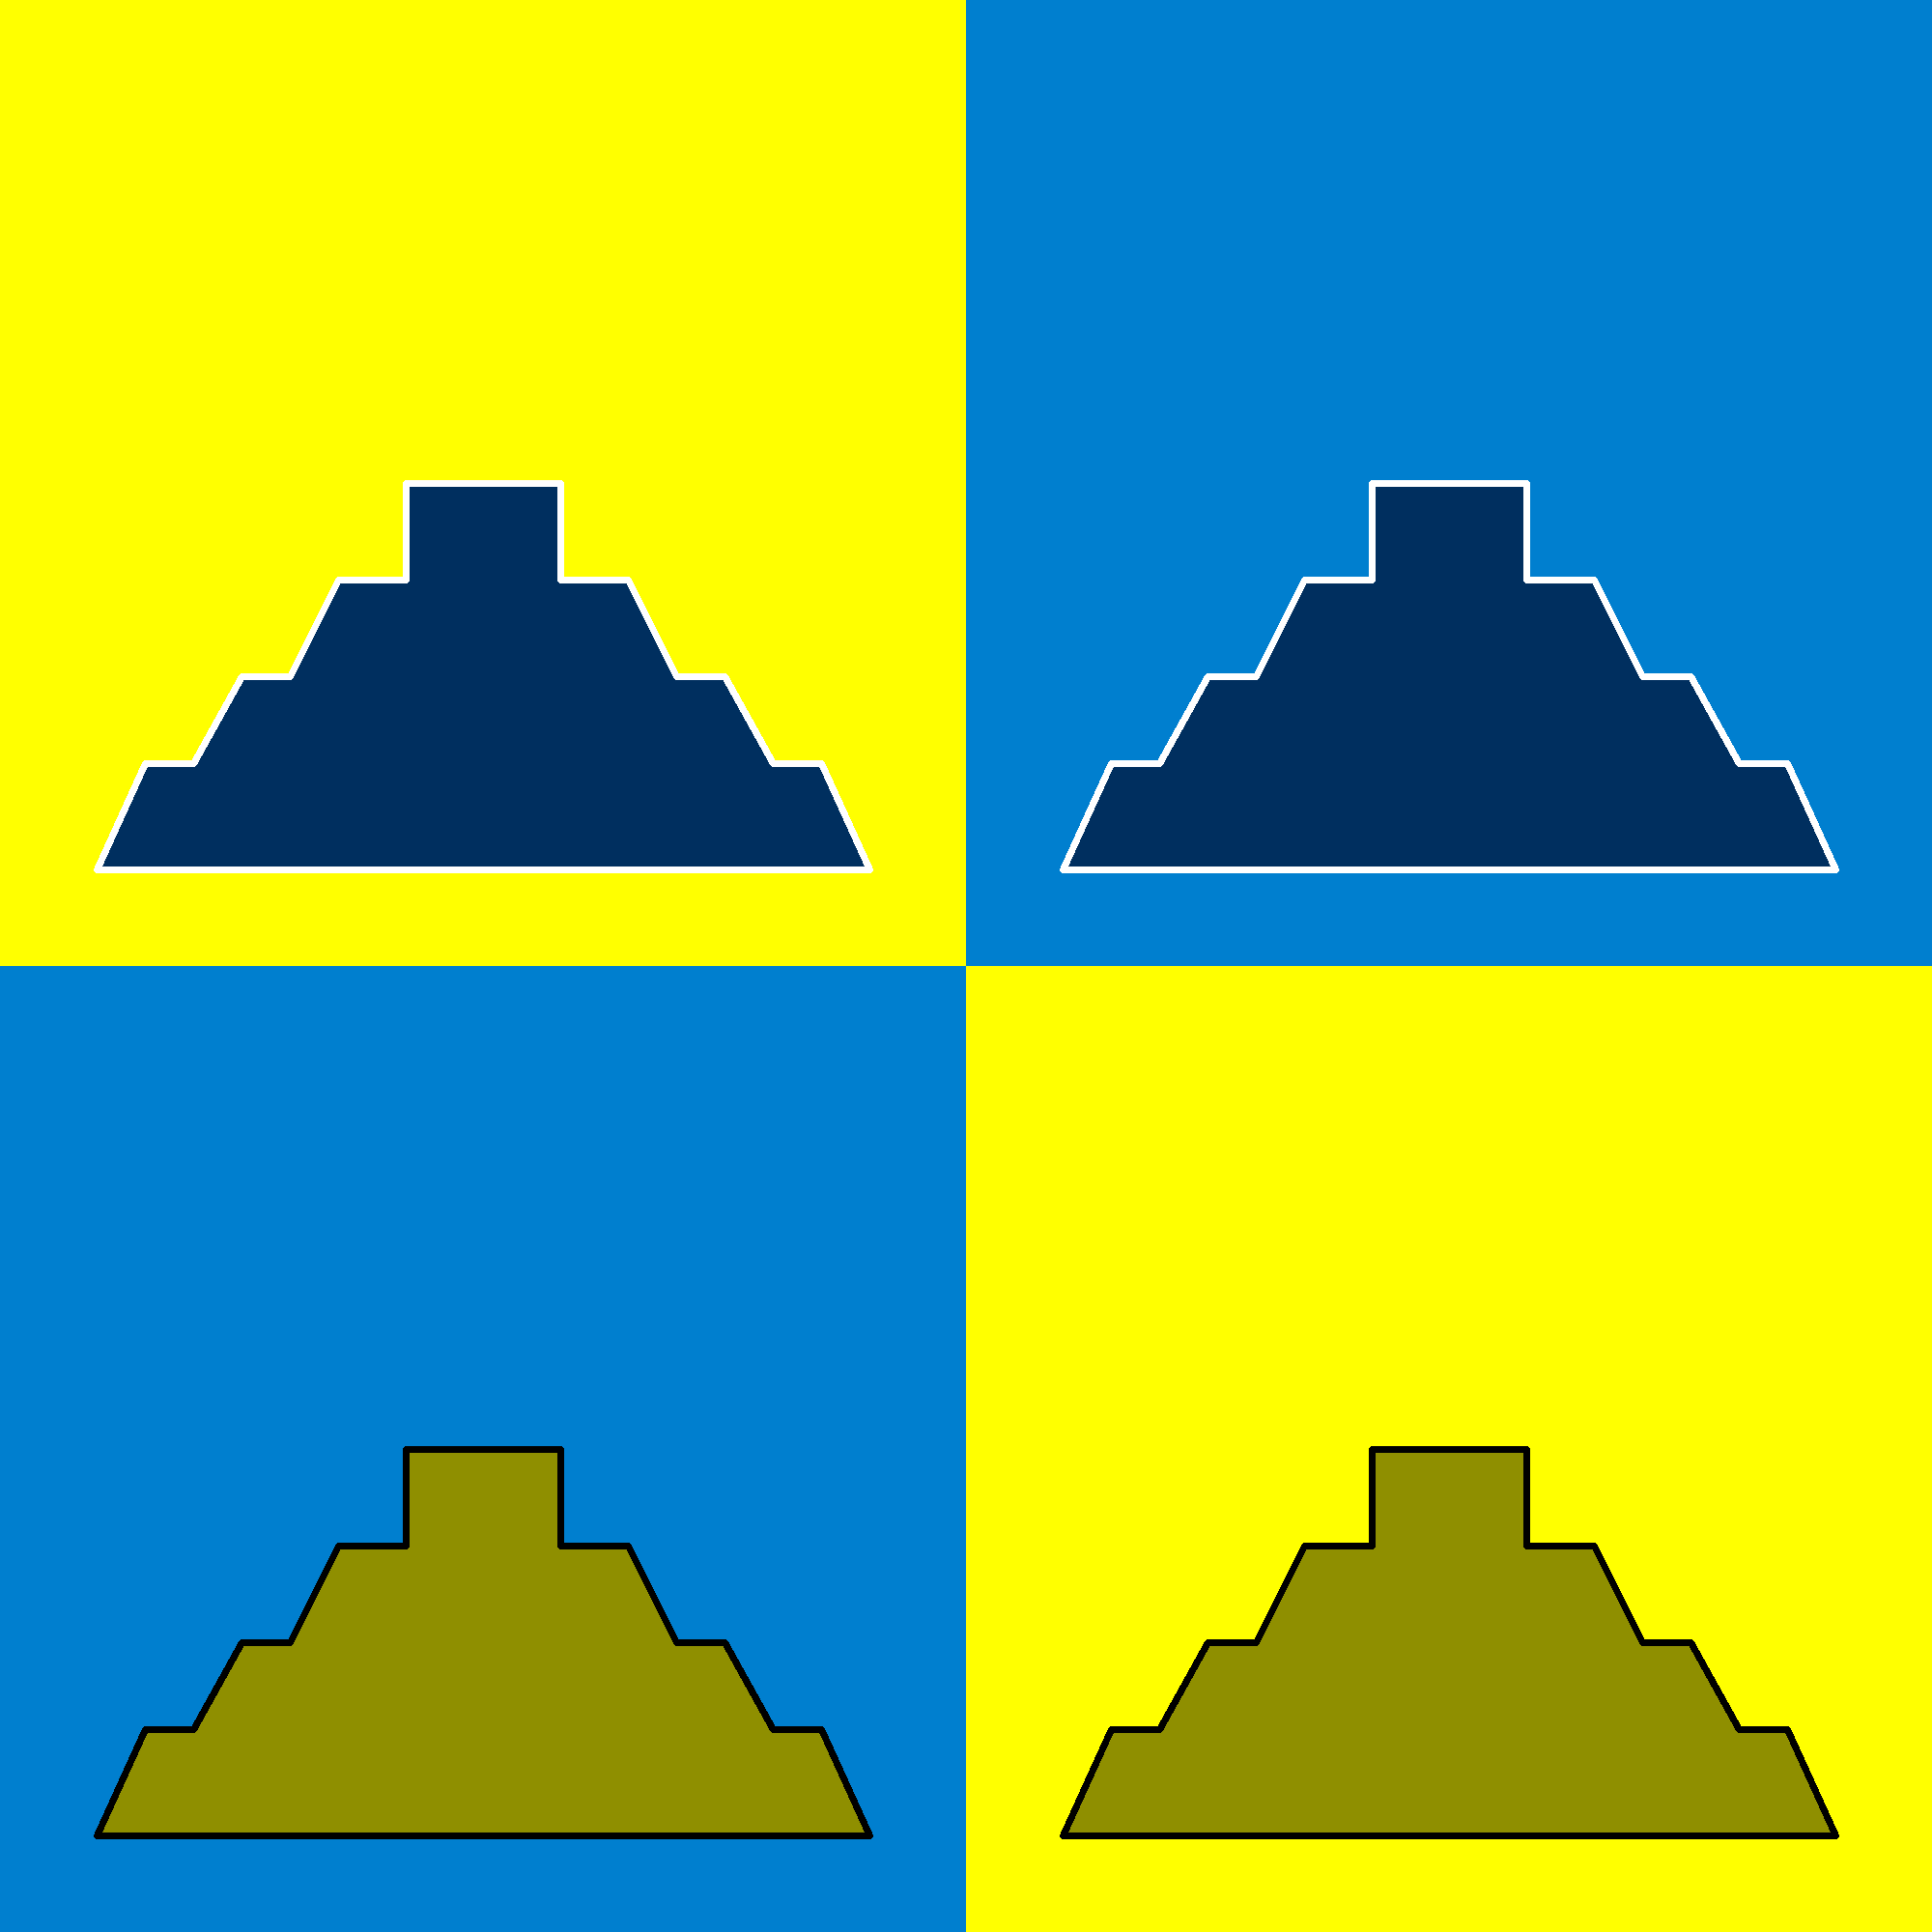
\includegraphics[width=0.4\textwidth, keepaspectratio=true]{pieces/08_pyramid.png}
\caption{Pyramid}
\label{fig:08_pyramid}
\end{wrapfigure}
Pyramid is passive piece, meaning it can't move on its own, it has to be
activated first. This is done by capturing a field at which Pyramid stands
with own other piece and then move Pyramid further.

Once activated, Pyramid moves similar to Rook, only real difference is that
it can move for only so many fields as piece activating it has moved, i.e.
for at most as momentum received.

\subsection*{Momentum}
\addcontentsline{toc}{subsection}{Momentum}

Momentum is count of fields traveled over by a piece. Pyramid receives
momentum from piece which activates it. Momentum is spent by Pyramid when
moving, one for each field travelled. So Pyramid can't move for more
fields than received momentum, i.e. for more than activating piece has
travelled. Momentum can't be saved for later, it is wasted when Pyramid
moves for less than received momentum.

Piece has momentum if it's equal to or greater than 1. Piece has no momentum
if it's 0. In all cases, momentum cannot become negative, it's not possible
to "borrow" momentum from activating piece to activated piece (Pyramid).

\clearpage % ..........................................................

\subsection*{Pyramid (cont.)}
\addcontentsline{toc}{subsection}{Pyramid (cont.)}

Pyramid can't check opponent's King, and consequently can't contribute to
checkmate. Pyramid can capture all the other opponent's pieces after it has
been activated, even if it has no remaining momentum, i.e. can't move any
further.

Pyramid can also promote own Pawns on
\hyperref[sec:Definitions/Sides of a chessboard]{opponent's side of the board}.
It can also convert any opponent's piece, except King, on
\hyperref[sec:Definitions/Sides of a chessboard]{own side of the board}.
To do either of these things, Pyramid does not have to have any remaining
momentum, it's enough if piece in question is within reach.

Pyramid can also activate other Pyramid, and transfer remaining momentum to it.
There has to be remaining momentum, it must be greater than 0 for cascading
to be permitted. Pyramid cannot activate any other piece, neither own nor
opponent's.

In algebraic notation symbol for Pyramid is 'A', to avoid confusion with Pawn.

\clearpage % ..........................................................
% Activation ----------------------------------------------------------

\subsection*{Activation}
\addcontentsline{toc}{subsection}{Activation}

\noindent
\begin{figure}[!h]
\includegraphics[width=1.0\textwidth, keepaspectratio=true]{examples/06_ma/scn_ma_01_pyramid_activation_init.png}
\caption{Pyramid activation}
\label{fig:scn_ma_01_pyramid_activation_init}
\end{figure}

Here Pegasus is about to capture field on which Pyramid stands. Note, only
step-fields are counted towards momentum. After activation Pyramid would be
limited to move at most 4 fields across, i.e. at most the momentum it received
from Pegasus.

\clearpage % ..........................................................

\noindent
\begin{figure}[!h]
\includegraphics[width=1.0\textwidth, keepaspectratio=true]{examples/06_ma/scn_ma_02_pyramid_activated.png}
\caption{Pyramid activated}
\label{fig:scn_ma_02_pyramid_activated}
\end{figure}

Above, arrows show all possible moves by Pyramid. Just like Rook, Pyramid has to
stop before own Bishop. Pyramid can capture opponent's Knight, but can't move any
further after capture. Pyramid can also capture opponent's Bishop, despite being
barely reachable.

% ---------------------------------------------------------- Activation
\clearpage % ..........................................................
% Promotion -----------------------------------------------------------

\subsection*{Promotion}
\addcontentsline{toc}{subsection}{Promotion}
\label{sec:Mayan Ascendancy/Pyramid/Promotion}

Pyramid can promote own Pawns, but only on opponent's side of the board.
Promotion is done by activating Pyramid which then marks Pawn for promotion
by touching either Pawn or field at which it stands. Pyramid then leaves
board as if captured by the opponent, and Pawn is replaced by desired piece,
for instance Queen.

Both Pyramid and Pawn in question has to reside on opponent's side of the
board before promotion can take place. Piece which activates Pyramid need
not to be on opponent's side of the board.

Piece which Pawn can be promoted to is from the set of all starting pieces,
except King. This promoting-to piece is not limited to pieces already being
captured.

\clearpage % ..........................................................

\noindent
\begin{figure}[!h]
\includegraphics[width=1.0\textwidth, keepaspectratio=true]{examples/06_ma/scn_ma_05_promo_init.png}
\caption{Promotion start}
\label{fig:scn_ma_05_promo_init}
\end{figure}

Here, Pegasus is accumulating momentum while travelling over step-fields. After
activation Pyramid would be limited to move at most 4 fields across, i.e. at most
the momentum it received from Pegasus.

\clearpage % ..........................................................

\noindent
\begin{figure}[!h]
\includegraphics[width=1.0\textwidth, keepaspectratio=true]{examples/06_ma/scn_ma_06_promo_pyramid_activated.png}
\caption{Promotion, Pyramid activated}
\label{fig:scn_ma_06_promo_pyramid_activated}
\end{figure}

Above, Pegasus captured field at which Pyramid was situated, arrows now show
all possible moves by Pyramid. Pyramid can't promote Pawn 2, as it is still
located on own half of the chessboard. Just as Rook, Pyramid can't advance
past Pawn 2. Only full movement to the right leads to promotion of Pawn 1,
shown in blue.

\clearpage % ..........................................................

\noindent
\begin{figure}[!h]
\includegraphics[width=1.0\textwidth, keepaspectratio=true]{examples/06_ma/scn_ma_07_promo_end.png}
\caption{Promotion end}
\label{fig:scn_ma_07_promo_end}
\end{figure}

Now that Pyramid has reached Pawn 1, it is removed from the board and piece of
choice, in this instance Queen, replaces Pawn. Just as with ordinary promotion,
this can take place regardless of which pieces has been captured, e.g. even if
own Queen is still present on chessboard.

% ----------------------------------------------------------- Promotion
\clearpage % ..........................................................
% Conversion ----------------------------------------------------------

\subsection*{Conversion}
\addcontentsline{toc}{subsection}{Conversion}
\label{sec:Mayan Ascendancy/Pyramid/Conversion}

Pyramid can convert opponent's pieces, except King, but only on own side of
the board. Conversion is done by activating Pyramid which then marks opponent's
piece for conversion by touching either piece or field at which it stands. Now
Pyramid leaves the board as if captured by the opponent, and opponent's piece
is replaced by own piece of the same type.

Both Pyramid and opponent's piece has to reside on own side of the board before
conversion can take place. Piece which activates Pyramid need not to be on own
side of the board. Conversion is not limited to pieces which has been captured.

Note that Pyramid might just as well capture opponent's piece. Differences are
what leaves chessboard, and what remains on captured field. Capture itself with
Pyramid is in no way different than that with Rook. In either case, converting
or capturing, it is enough if Pyramid can reach opponent's piece, i.e. has
enough momentum.

\clearpage % ..........................................................

\noindent
\begin{figure}[!h]
\includegraphics[width=1.0\textwidth, keepaspectratio=true]{examples/06_ma/scn_ma_08_conversion_init.png}
\caption{Conversion start}
\label{fig:scn_ma_08_conversion_init}
\end{figure}

In example above, Bishop is travelling over 4 step-fields to reach for Pyramid,
and so that is momentum Pyramid will receive when activated by the Bishop.
This is also limit how far Pyramid could move after being activated.

\clearpage % ..........................................................

\noindent
\begin{figure}[!h]
\includegraphics[width=1.0\textwidth, keepaspectratio=true]{examples/06_ma/scn_ma_09_conversion_pyramid_activated.png}
\caption{Conversion, Pyramid activated}
\label{fig:scn_ma_09_conversion_pyramid_activated}
\end{figure}

Above, Bishop captured field at which Pyramid was situated, arrows now show all
possible moves by Pyramid. Pyramid can't convert opponent's Bishop, as it is still
located on opponent's side of chessboard. Pyramid could capture opponent's Bishop.
Again, just like Rook, Pyramid can't advance past opponent's Bishop. Only full
movement to the right leads to conversion of opponent's Rook, shown in blue.

\clearpage % ..........................................................

\noindent
\begin{figure}[!h]
\includegraphics[width=1.0\textwidth, keepaspectratio=true]{examples/06_ma/scn_ma_10_conversion_end.png}
\caption{Conversion end}
\label{fig:scn_ma_10_conversion_end}
\end{figure}

Now that Pyramid has reached opponent's Rook, it is removed from the board and
own Rook replaces opponent's Rook. This conversion can still take place, regardless
if any light Rook has been captured or not, i.e. even with both light Rooks still
present on chessboard. Capturing opponent's Rook would simply leave Pyramid in
place of it.

\clearpage % ..........................................................

\subsubsection*{Converting Rooks}
\addcontentsline{toc}{subsubsection}{Converting Rooks}
\label{sec:Mayan Ascendancy/Pyramid/Conversion/Converting Rooks}

\huge
TODO
\normalsize

\clearpage % ..........................................................

\subsubsection*{Converting Pawns}
\addcontentsline{toc}{subsubsection}{Converting Pawns}
\label{sec:Mayan Ascendancy/Pyramid/Conversion/Converting Pawns}

\huge
TODO
\normalsize

% ---------------------------------------------------------- Conversion
\clearpage % ..........................................................
% Cascading -----------------------------------------------------------

\subsection*{Cascading}
\addcontentsline{toc}{subsection}{Cascading}

\noindent
\begin{figure}[!h]
\includegraphics[width=1.0\textwidth, keepaspectratio=true]{examples/06_ma/scn_ma_11_cascading_init.png}
\caption{Cascading start}
\label{fig:scn_ma_11_cascading_init}
\end{figure}

Once activated, Pyramid can also activate another Pyramid. To do so, activated
Pyramid has to have at least 1 remaining momentum to transfer it to another
Pyramid. If all momentum received was spent moving, Pyramid cannot cascade, i.e.
cannot activate another Pyramid.

\clearpage % ..........................................................

\noindent
\begin{figure}[!h]
\includegraphics[width=1.0\textwidth, keepaspectratio=true]{examples/06_ma/scn_ma_12_cascading_pyramid_1_activated.png}
\caption{Cascading, 1st Pyramid activated}
\label{fig:scn_ma_12_cascading_pyramid_1_activated}
\end{figure}

Pyramid 1 has been activated by Queen and received momentum of 5, arrows now show
its all possible moves. Note, Pyramid 3 can't be activated, it's on the very end
of fields reachable by Pyramid 1. Note also that Pyramid 1 can't activate, nor move
past light Bishop on the left.

\clearpage % ..........................................................

\noindent
\begin{figure}[!h]
\includegraphics[width=1.0\textwidth, keepaspectratio=true]{examples/06_ma/scn_ma_13_cascading_pyramid_2_activated.png}
\caption{Cascading, 2nd Pyramid activated}
\label{fig:scn_ma_13_cascading_pyramid_2_activated}
\end{figure}

Pyramid 2 has been activated by Pyramid 1 and in the process received momentum of 2,
arrows now show all possible moves by Pyramid 2.

\clearpage % ..........................................................

\noindent
\begin{figure}[!h]
\includegraphics[width=1.0\textwidth, keepaspectratio=true]{examples/06_ma/scn_ma_14_cascading_end.png}
\caption{Cascading end}
\label{fig:scn_ma_14_cascading_end}
\end{figure}

Pyramid 2 has finished its movement, and so it ends light player's complete move,
which consisted of 3 plies, i.e. 3 pieces has been moved.

% ----------------------------------------------------------- Cascading
\clearpage % ..........................................................

\subsection*{Against King}
\addcontentsline{toc}{subsection}{Against King}

Pyramid can't check opponent's King, meaning that King is not under check even if
Pyramid could capture any other piece on the same field.

\noindent
\begin{figure}[!h]
\includegraphics[width=1.0\textwidth, keepaspectratio=true]{examples/06_ma/scn_ma_15_pyramid_vs_king.png}
\caption{Pyramid vs. King}
\label{fig:scn_ma_15_pyramid_vs_king}
\end{figure}

Above, King does not have to move/defend, as it is not under check from Pyramid.

\noindent
\begin{figure}[!h]
\includegraphics[width=1.0\textwidth, keepaspectratio=true]{examples/06_ma/scn_ma_16_pyramid_vs_bishop.png}
\caption{Pyramid vs. Bishop}
\label{fig:scn_ma_16_pyramid_vs_bishop}
\end{figure}

Bishop in the same place, however, could be captured without any hindrance.

\clearpage % ..........................................................

\subsection*{Activation by Pawn}
\addcontentsline{toc}{subsection}{Activation by Pawn}

\noindent
\begin{figure}[!h]
\includegraphics[width=1.0\textwidth, keepaspectratio=true]{examples/06_ma/scn_ma_04_pyramid_activation_by_pawn.png}
\caption{Pyramid activation by Pawns}
\label{fig:scn_ma_04_pyramid_activation_by_pawn}
\end{figure}

Pawns can activate Pyramid on own capture-field giving it 1 momentum, see Pawn 1.
Pawns can't activate Pyramids on step-fields, and are blocked from moving further,
see Pawns 2 and 3.

% ************************************************************* Pyramid
\clearpage % ..........................................................

\section*{Rush, en passant}
\addcontentsline{toc}{section}{Rush, en passant}

\noindent
\begin{wrapfigure}{l}{0.4\textwidth}
\centering
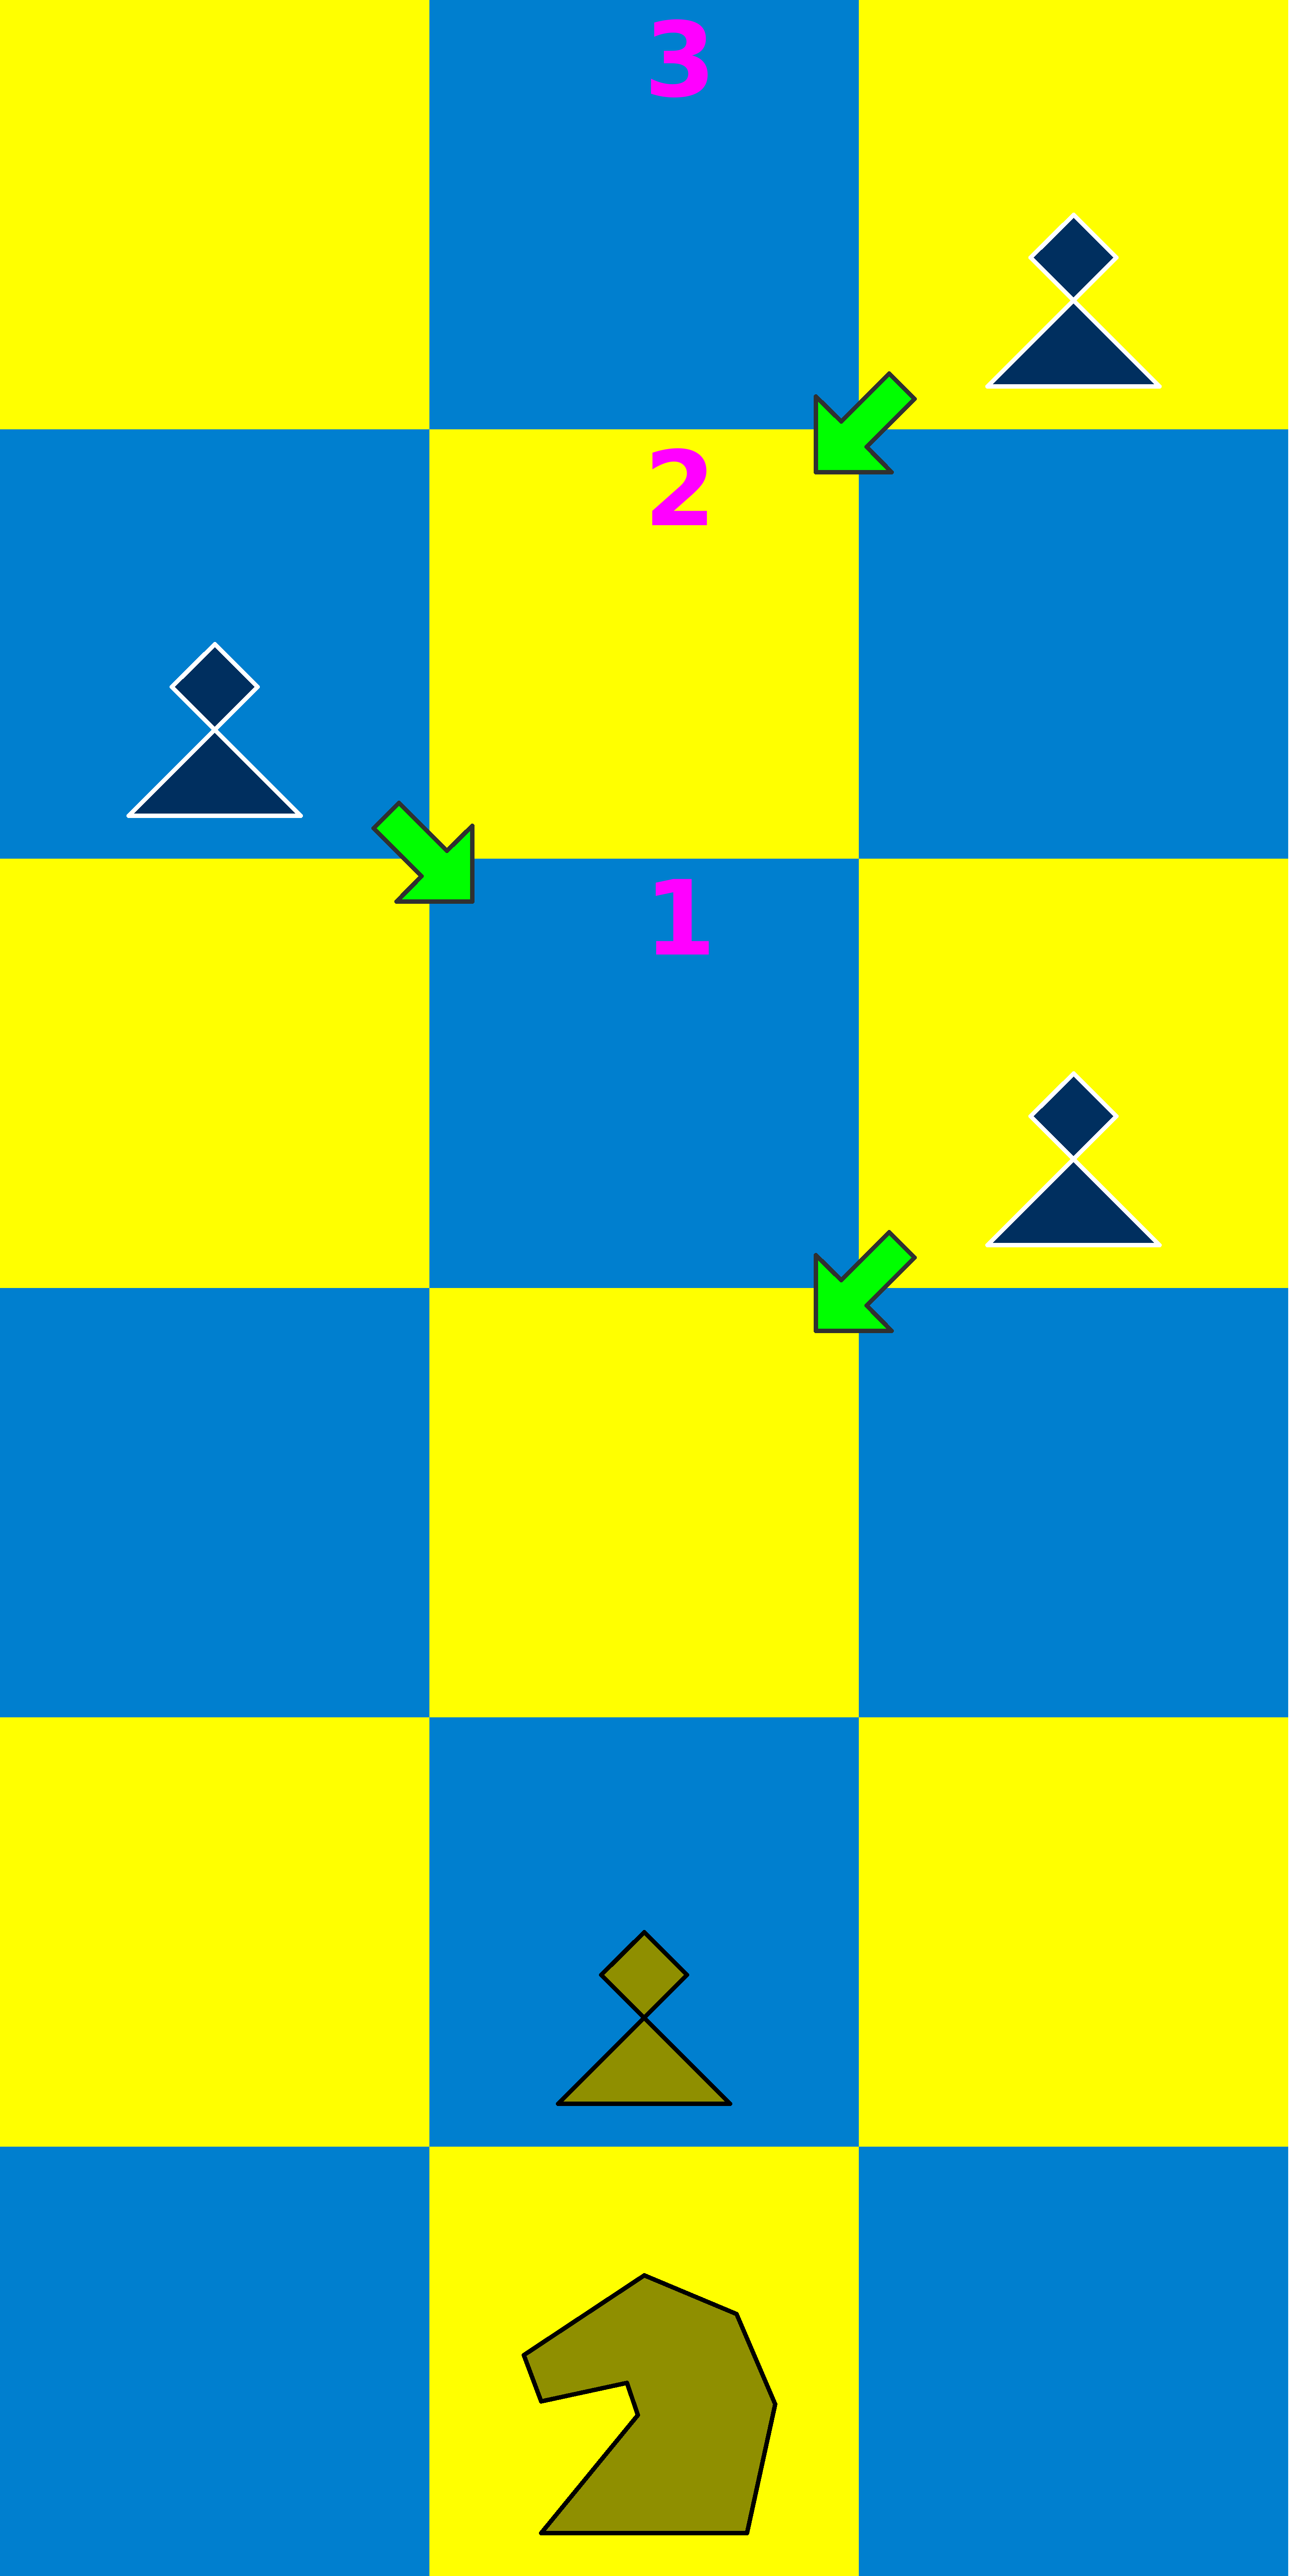
\includegraphics[width=0.25\textwidth, keepaspectratio=true]{en_passants/06_mayan_ascendancy_en_passant.png}
\caption{En passant}
\label{fig:06_mayan_ascendancy_en_passant}
\end{wrapfigure}
Rush and en passant are identical to those in Classic Chess, only difference
is that Pawn can now move longer on initial turn, up to 4 fields in this
variant.

Converted opponent's Pawns cannot be rushed, even if converted on an initial positions
of own Pawns.

\clearpage % ..........................................................

\section*{Castling}
\addcontentsline{toc}{section}{Castling}

Castling is the same as in Classical Chess, only difference is that King can move 2, 3 or 4 fields across.
All other constraints from Classical Chess still applies.

\noindent
\begin{figure}[!h]
\includegraphics[width=1.0\textwidth, keepaspectratio=true]{castlings/06_ma/mayan_ascendancy_castling.png}
\caption{Castling}
\label{fig:mayan_ascendancy_castling}
\end{figure}

In example above, all valid King's castling moves are numbered. After any castling, Rook
ends on a field next to King closer to center, i.e. closer to King's initial position.

\noindent
\begin{figure}[!h]
\includegraphics[width=1.0\textwidth, keepaspectratio=true]{castlings/06_ma/mayan_ascendancy_castling_right_04.png}
\caption{Castling long right}
\label{fig:mayan_ascendancy_castling_right_04}
\end{figure}

In this example King was castling long to the right. Initial King's position is marked with "K".
After castling is finished, right Rook ends up on the field immediately left to the King.

Converted opponent's Rooks cannot be castled, even if converted on an initial positions
of own Rooks.

\clearpage % ..........................................................

\section*{Initial setup}
\addcontentsline{toc}{section}{Initial setup}

Compared to initial setup of Croatian Ties, Pyramid is inserted between Pegasus and Knight
symmetrically, on both sides of chessboard. This can be seen in the image below:

\noindent
\begin{figure}[h]
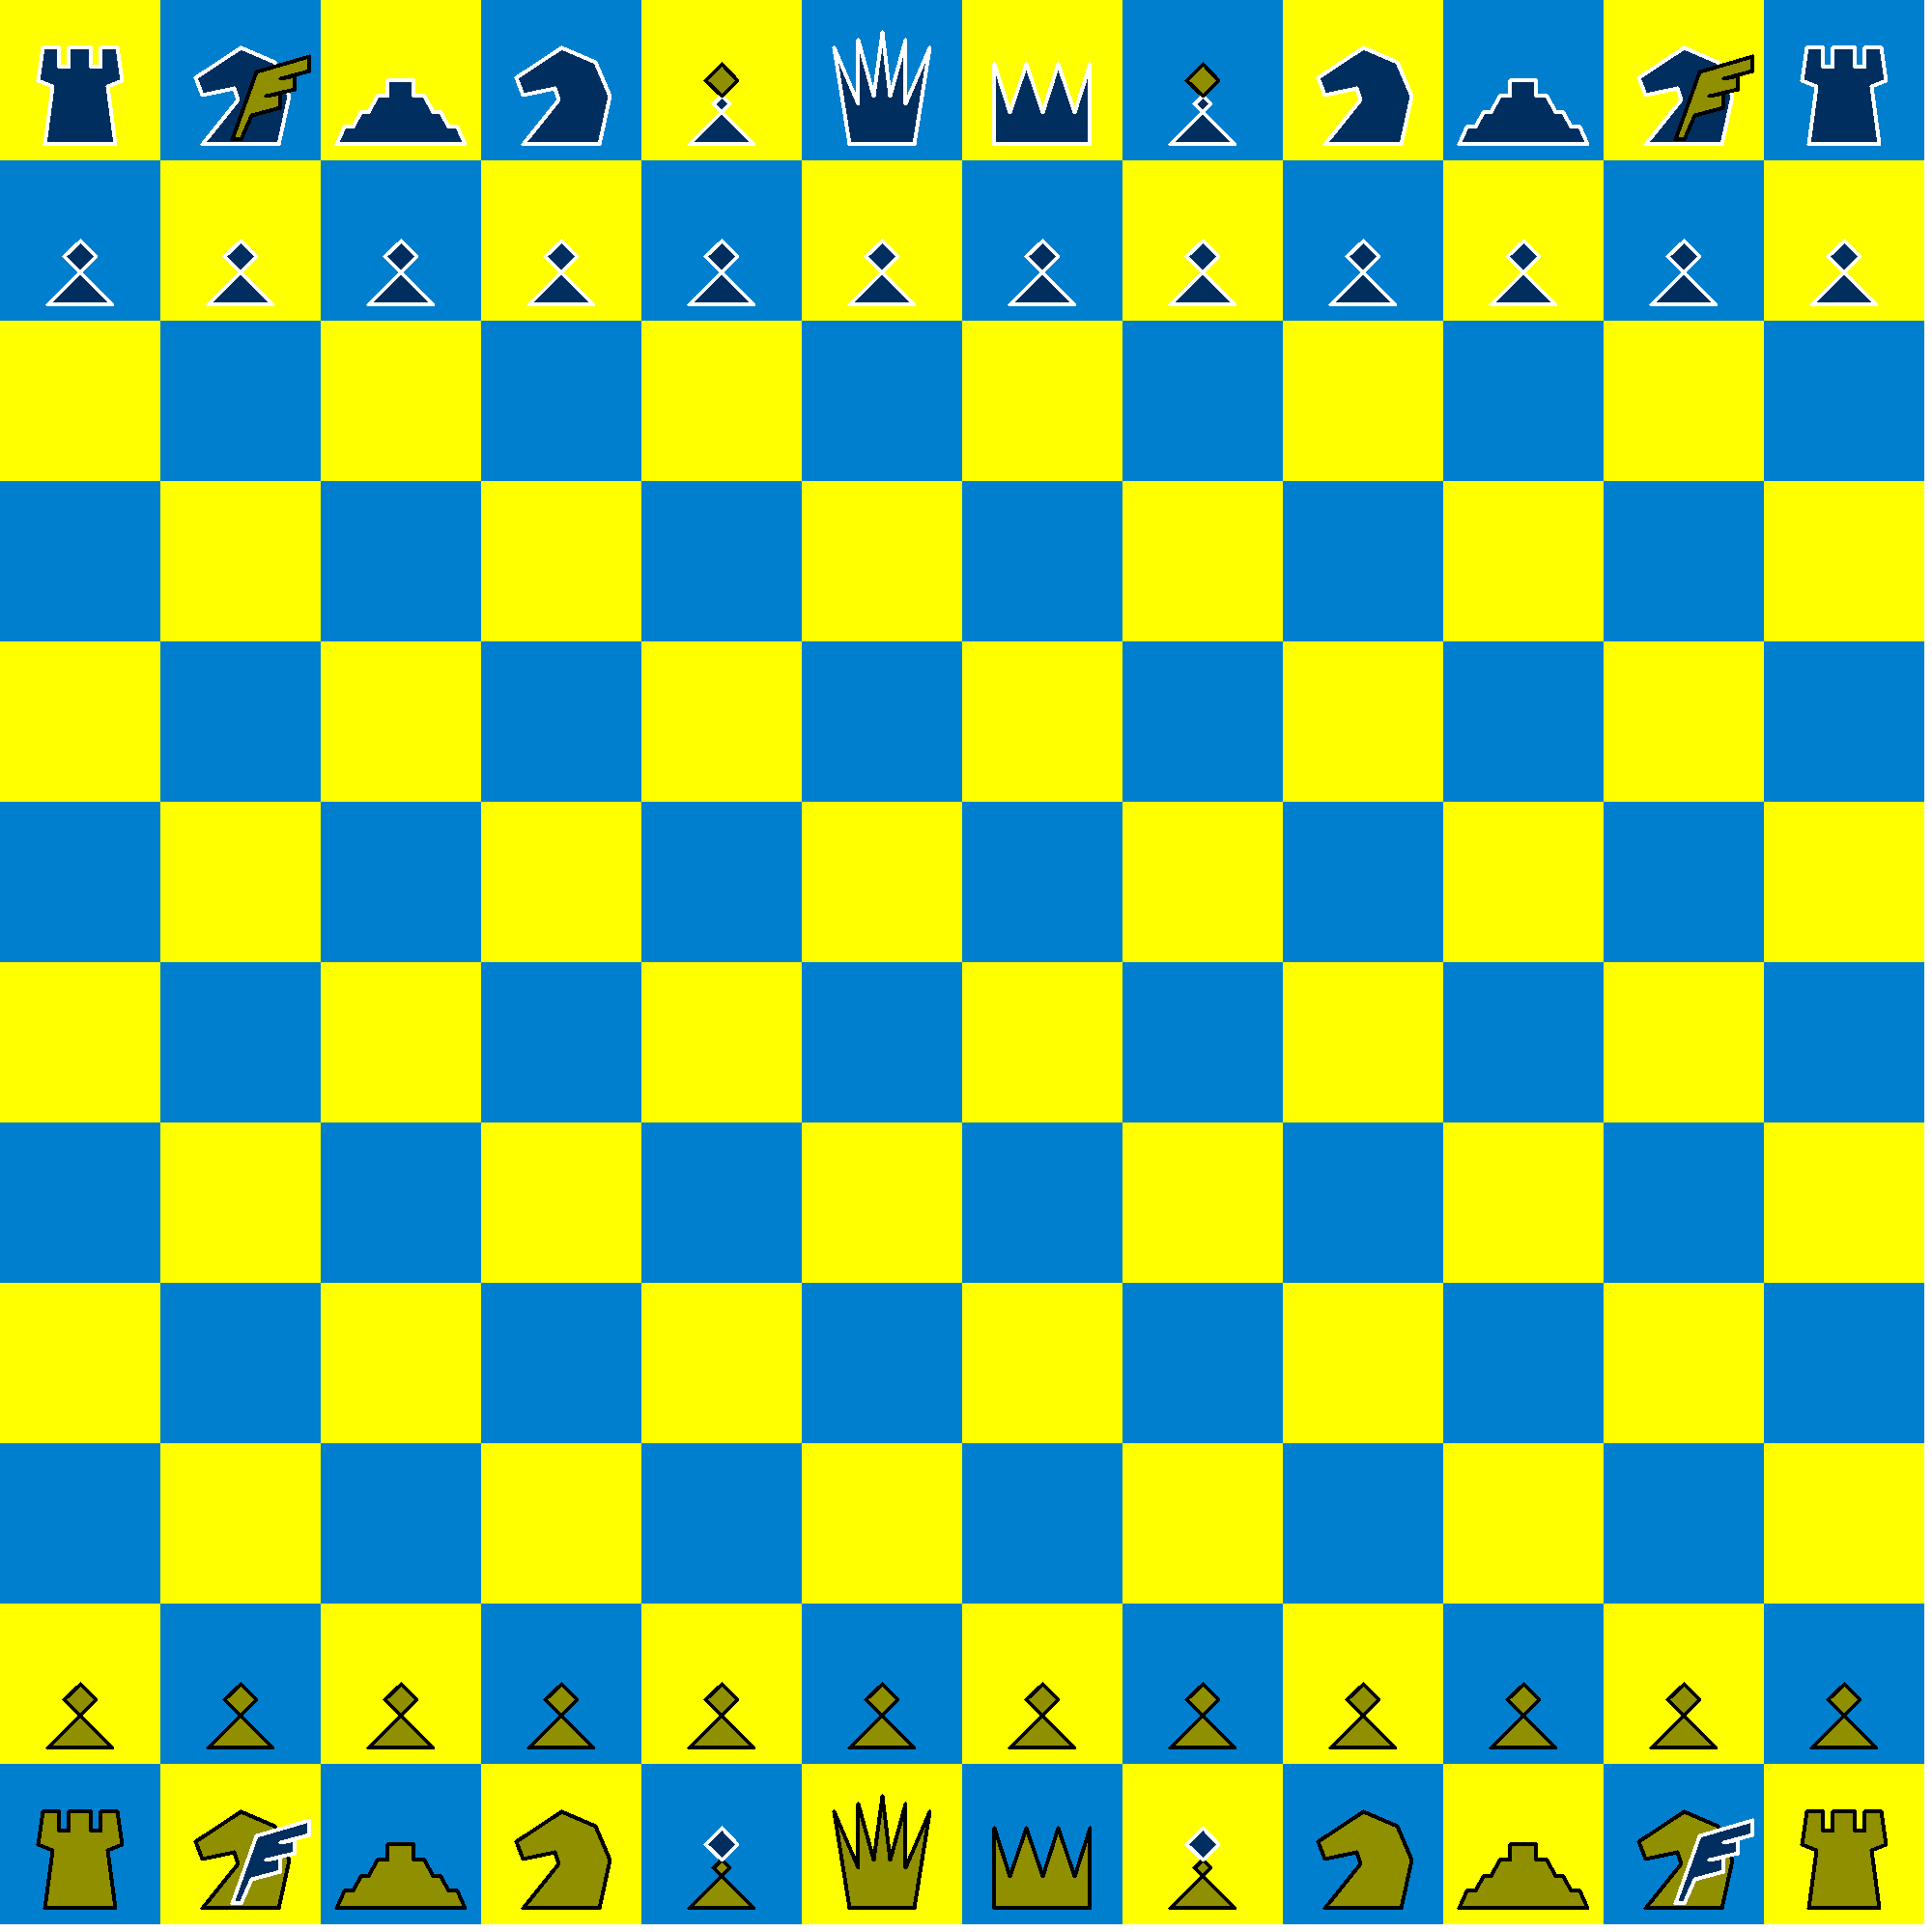
\includegraphics[width=1.0\textwidth, keepaspectratio=true]{boards/06_mayan_ascendancy.png}
\caption{Mayan Ascendancy board}
\label{fig:06_mayan_ascendancy}
\end{figure}

\clearpage % ..........................................................
% ============================================ Mayan Ascendancy chapter
